%-- Template based off http://www.latextemplates.com/template/structured-general-purpose-assignment.

%%%%%%%%%%%%%%%%%%%%%%%%%%%%%%%%%%%%%%%%%
% Structured General Purpose Assignment
% LaTeX Template
%
% This template has been downloaded from:
% http://www.latextemplates.com
%
% Original author:
% Ted Pavlic (http://www.tedpavlic.com)
%
% Note:
% The \lipsum[#] commands throughout this template generate dummy text
% to fill the template out. These commands should all be removed when 
% writing assignment content.
%
%%%%%%%%%%%%%%%%%%%%%%%%%%%%%%%%%%%%%%%%%

%----------------------------------------------------------------------------------------
%	PACKAGES AND OTHER DOCUMENT CONFIGURATIONS
%----------------------------------------------------------------------------------------

\documentclass{article}

\usepackage{fancyhdr} % Required for custom headers
\usepackage{lastpage} % Required to determine the last page for the footer
\usepackage{extramarks} % Required for headers and footers
\usepackage{graphicx} % Required for including pictures
\usepackage{biblatex}
\usepackage{caption}
\usepackage{float}
\usepackage[none]{hyphenat}
\usepackage{hyperref}


\bibliography{main.bib}
\graphicspath{ {images/} }

% Margins
\topmargin=-0.45in
\evensidemargin=0in
\oddsidemargin=0in
\textwidth=6.5in
\textheight=9.0in
\headsep=0.25in 

\linespread{1.1} % Line spacing

% Set up the header and footer
\pagestyle{fancy}
\lhead{\hmwkTitle} % Top left header
\chead{\hmwkShortCode} % Top center header
\rhead{\hmwkAuthorName} % Top right header
\lfoot{\lastxmark} % Bottom left footer
\cfoot{} % Bottom center footer
\rfoot{Page\ \thepage\ of\ \pageref{LastPage}} % Bottom right footer
\renewcommand\headrulewidth{0.4pt} % Size of the header rule
\renewcommand\footrulewidth{0.4pt} % Size of the footer rule

\setlength\parindent{0pt} % Removes all indentation from paragraphs

%----------------------------------------------------------------------------------------
%	DOCUMENT STRUCTURE COMMANDS
%	Skip this unless you know what you're doing
%----------------------------------------------------------------------------------------

% Header and footer for when a page split occurs within a problem environment
\newcommand{\enterProblemHeader}[1]{
\nobreak\extramarks{#1}{#1 continued on next page\ldots}\nobreak
\nobreak\extramarks{#1 (continued)}{#1 continued on next page\ldots}\nobreak
}

% Header and footer for when a page split occurs between problem environments
\newcommand{\exitProblemHeader}[1]{
\nobreak\extramarks{#1 (continued)}{#1 continued on next page\ldots}\nobreak
\nobreak\extramarks{#1}{}\nobreak
}

\setcounter{secnumdepth}{0} % Removes default section numbers
\newcounter{homeworkProblemCounter} % Creates a counter to keep track of the number of problems

\newcommand{\homeworkProblemName}{}
\newenvironment{homeworkProblem}[1][Problem \arabic{homeworkProblemCounter}]{ % Makes a new environment called homeworkProblem which takes 1 argument (custom name) but the default is "Problem #"
\stepcounter{homeworkProblemCounter} % Increase counter for number of problems
\renewcommand{\homeworkProblemName}{#1} % Assign \homeworkProblemName the name of the problem
\section{\homeworkProblemName} % Make a section in the document with the custom problem count
\enterProblemHeader{\homeworkProblemName} % Header and footer within the environment
}{
\exitProblemHeader{\homeworkProblemName} % Header and footer after the environment
}

\newcommand{\problemAnswer}[1]{ % Defines the problem answer command with the content as the only argument
\noindent\framebox[\columnwidth][c]{\begin{minipage}{0.98\columnwidth}#1\end{minipage}} % Makes the box around the problem answer and puts the content inside
}

\newcommand{\homeworkSectionName}{}
\newenvironment{homeworkSection}[1]{ % New environment for sections within homework problems, takes 1 argument - the name of the section
\renewcommand{\homeworkSectionName}{#1} % Assign \homeworkSectionName to the name of the section from the environment argument
\subsection{\homeworkSectionName} % Make a subsection with the custom name of the subsection
\enterProblemHeader{\homeworkProblemName\ [\homeworkSectionName]} % Header and footer within the environment
}{
\enterProblemHeader{\homeworkProblemName} % Header and footer after the environment
}
   
%----------------------------------------------------------------------------------------
%	NAME AND CLASS SECTION
%----------------------------------------------------------------------------------------

\newcommand{\hmwkTitle}{Enhancing the CS-Alumni Application} % Assignment title
\newcommand{\hmwkDueDate}{Monday,\ Decemeber\ 8,\ 2014} % Due date
\newcommand{\hmwkShortCode}{SE31520}
\newcommand{\hmwkClass}{Developing Internet-Based Applications} % Course/class
\newcommand{\hmwkClassTime}{4pm} % Class/lecture time
\newcommand{\hmwkAuthorName}{Thomas Mark Rosier (THR2)} % Your name
\newcommand{\hmwkStudentId}{110113188} % Student ID

%----------------------------------------------------------------------------------------
%	TITLE PAGE
%----------------------------------------------------------------------------------------

\title{
\vspace{2in}
\textmd{\textbf{\hmwkShortCode\\ \hmwkClass}}\\
\normalsize
\vspace{0.1in}
\textbf{\hmwkTitle}\\
\vspace{0.1in}
\small{Submission\ Due\ \hmwkClassTime\ \hmwkDueDate}\\
\vspace{3in}
}

\author{
\textbf{\hmwkAuthorName}\\
\hmwkStudentId
}
\date{} % Insert date here if you want it to appear below your name

%----------------------------------------------------------------------------------------

\begin{document}

\maketitle

%----------------------------------------------------------------------------------------
%	TABLE OF CONTENTS
%----------------------------------------------------------------------------------------

%\setcounter{tocdepth}{1} % Uncomment this line if you don't want subsections listed in the ToC

\newpage
\tableofcontents
\newpage


\nocite{bara:2013:online}
\nocite{saa:2013:online}

%-- Document Summary.
\section{Document Summary}

\iffalse
 _________    ________      ________      ________     
|\___   ___\ |\   __  \    |\   ___ \    |\   __  \    
\|___ \  \_| \ \  \|\  \   \ \  \_|\ \   \ \  \|\  \   
     \ \  \   \ \  \\\  \   \ \  \ \\ \   \ \  \\\  \  
      \ \  \   \ \  \\\  \   \ \  \_\\ \   \ \  \\\  \ 
       \ \__\   \ \_______\   \ \_______\   \ \_______\
        \|__|    \|_______|    \|_______|    \|_______|                                               
\fi   

%-- Application Design.
\section{Application Design}

\subsection{CS-Alumni Chrome Browser Extension}

\subsubsection{Rational}

My rational behind deciding to develop a browser extension for this project, was that this has been a technology that I have been following for a while and I have not seen it used that regularly for small little applications that interface with a bigger application.\\
\\
Another reason for my choice to develop a browser extension was that I wanted to learn about implementing some of the more advanced features within the Chrome SDK; for example the use of 'Background Pages' which are used to keep a task running in the background while the extension is closed.\\
\\
One of the newer features within the Chrome SDK that had also caught my attention in the weeks before starting this assignment was the use of Chrome desktop notifications where you can create a notification within your application that will be displayed to the end user via the Chrome UI's notification draw.\\
\\
I wanted to see if it was possible to encapsulate some of the key management features of the CS-Alumni application into an attractive and well presented browser extension that also notified the user of any new broadcasts that had been made.\\
\\
Why did I choose to develop a Chrome extension over a Firefox, Safari or Internet Explorer? The main reason was due to Chris Loftus's preference of Chrome over the other browsers. In addition to that I felt that due to developing for Chrome this also meant that the code will work without modification in Opera. This is a bonus in the real world as it means we can support a greater population of users without investing more money into development.\\
\\
I also feel that Chrome has a much nicer development environment for developing browser extensions over its competitors, along with having some newer and more unique features that allow the Chrome based extension to stand out.\\
\\
If this was a real world product it would not take many resources to port the extension to work on Firefox and Safari as well, but this was not within the scope of this assignment.

\newpage
\subsubsection{Module Diagrams}

\iffalse
 _________    ________      ________      ________     
|\___   ___\ |\   __  \    |\   ___ \    |\   __  \    
\|___ \  \_| \ \  \|\  \   \ \  \_|\ \   \ \  \|\  \   
     \ \  \   \ \  \\\  \   \ \  \ \\ \   \ \  \\\  \  
      \ \  \   \ \  \\\  \   \ \  \_\\ \   \ \  \\\  \ 
       \ \__\   \ \_______\   \ \_______\   \ \_______\
        \|__|    \|_______|    \|_______|    \|_______|                                               
\fi                                                   


\newpage
\subsubsection{Program Operation}

When the user opens the browser extension they will be presented with the home screen. This shows a brief summary about the application along with a disclaimer.\\
\\
Due to this being an assignment this is essentially a development version of the browser extension. So I have included a link to the Unit tests on the home page to make it easily accessible during the development and testing of the application. If this extension was intended to be released as production code this link would be removed or turned off within the configuration.\\

\begin{figure}[H]
\centering
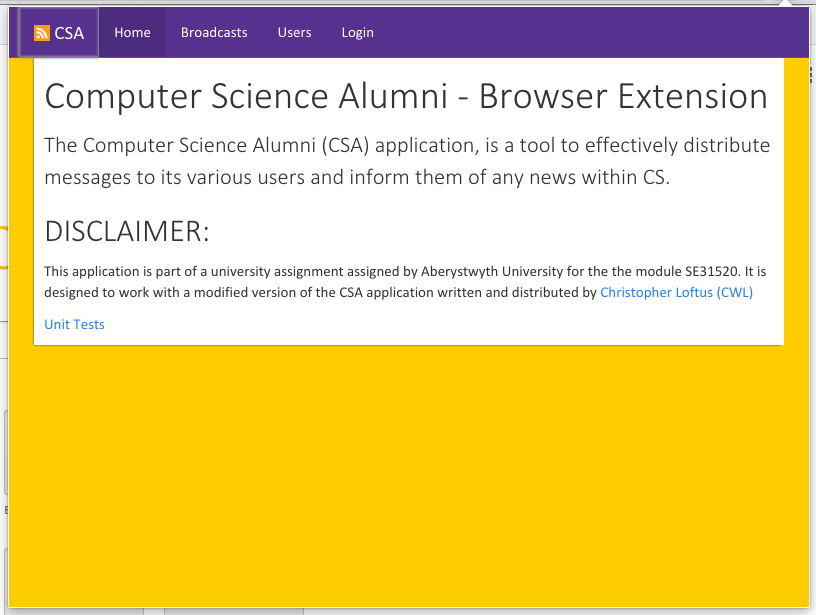
\includegraphics[width=0.7\textwidth]{homepage}
\caption{The screenshot above is the landing screen for the browser extension.}
\end{figure}

\newpage
From the home page the user can navigate to the 'Broadcasts' tab. In the figure captioned there is no broadcasts available to the user so they are shown a message that says that there are no broadcasts.\\

\begin{figure}[H]
\centering
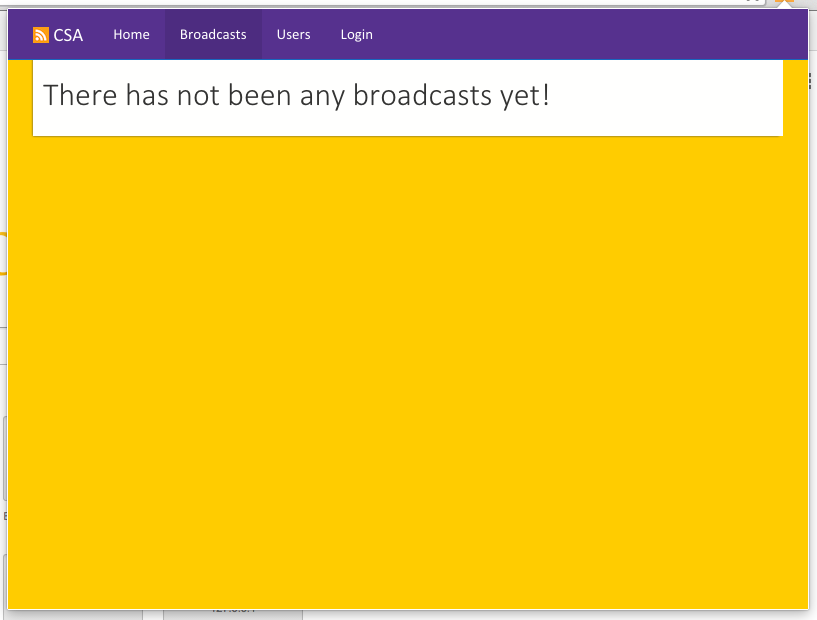
\includegraphics[width=0.7\textwidth]{bcpage}
\caption{Above we see the broadcasts screen with no broadcasts available.}
\end{figure}

Again below we see the 'Broadcasts' tab. This time we see how the page appears when there are broadcasts.

\begin{figure}[H]
\centering
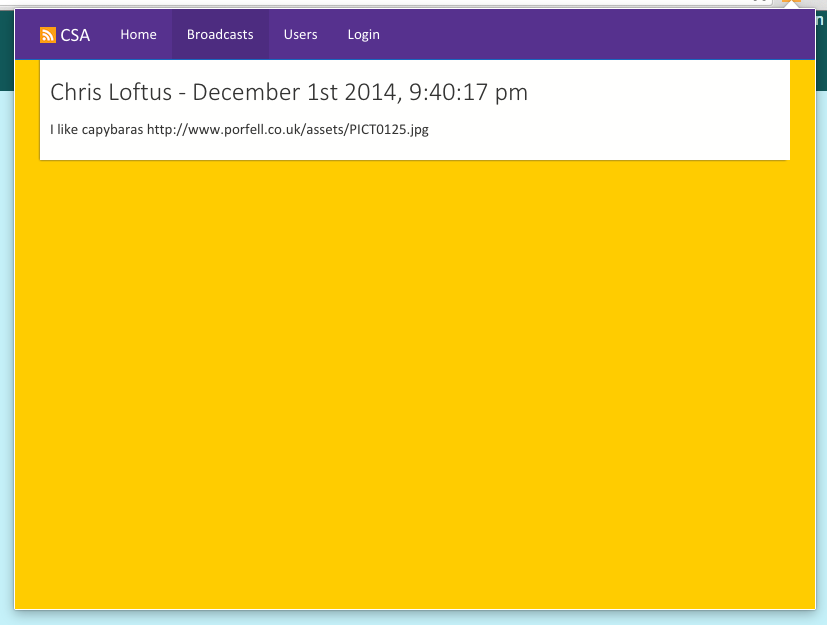
\includegraphics[width=0.7\textwidth]{populatebcpage}
\caption{This is what the populated broadcast screen looks like.}
\end{figure}

This is the 'users' tab of the browser extension where the user can view a specific user's details and edit their information if it is deemed appropriate.

\begin{figure}[H]
\centering
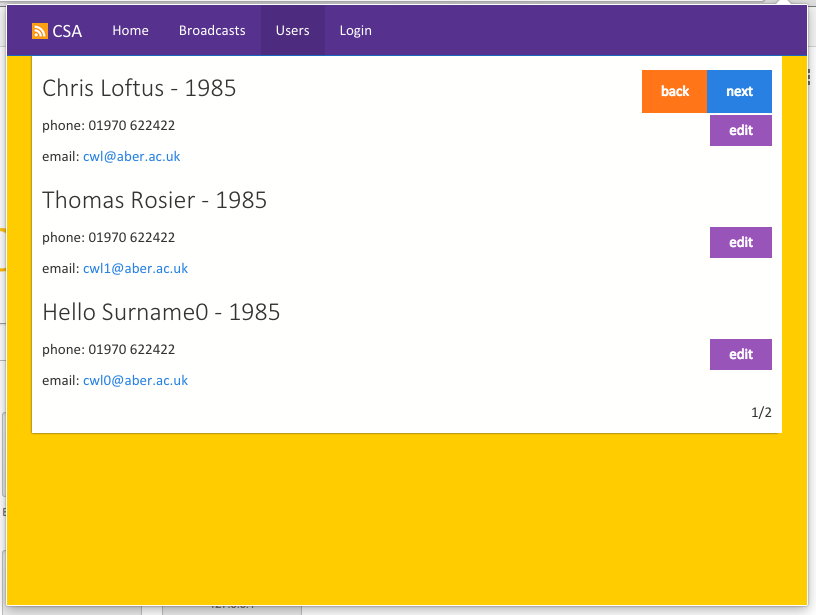
\includegraphics[width=0.7\textwidth]{userpage}
\caption{Here we have a screenshot of the user's screen.}
\end{figure}

When the edit button has been selected for a specific user it shows this modal window that allows the user to edit the details that are kept on the current user they are editing.

\begin{figure}[H]
\centering
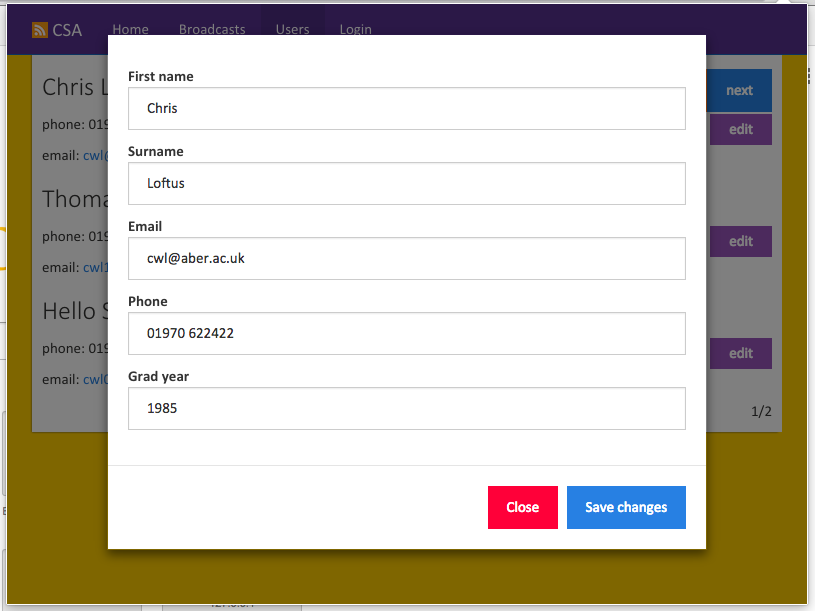
\includegraphics[width=0.7\textwidth]{modalpage}
\caption{Above we have a screenshot showing the modal window we used to edit the user information.}
\end{figure}

\newpage
The 'Login' tab is where the user enters there login credentials that will be used to authenticate the user against the CS-Alumni application.

\begin{figure}[H]
\centering
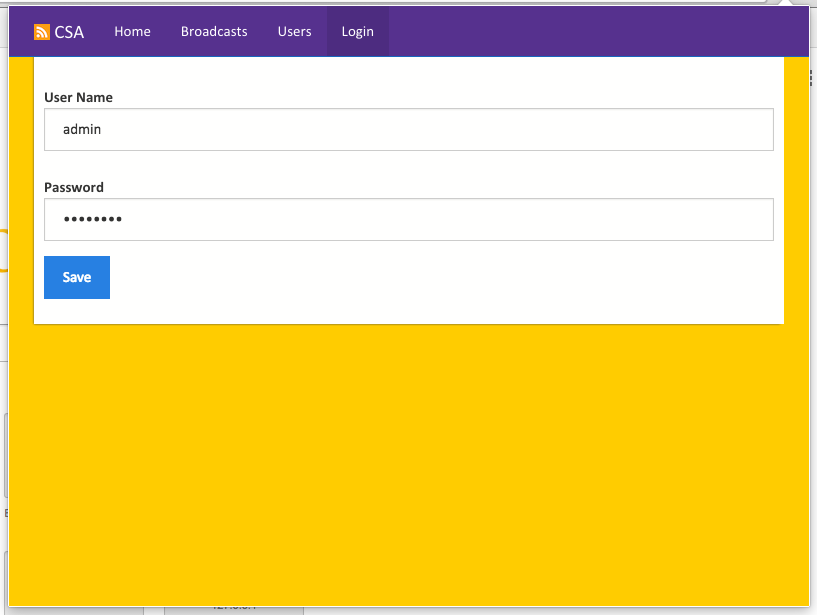
\includegraphics[width=0.7\textwidth]{loginpage}
\caption{This is a screenshot of the login screen.}
\end{figure}

In the screenshot below I have created a new broadcast within the CS-Alumni application to showcase the notification features within the browser extension.\\
\\
Note: The destination list differs from the standard CSA application. They have been modified to remove the networks that do not work along with adding in the functionality to target the browser extension specifically.\\

\begin{figure}[H]
\centering
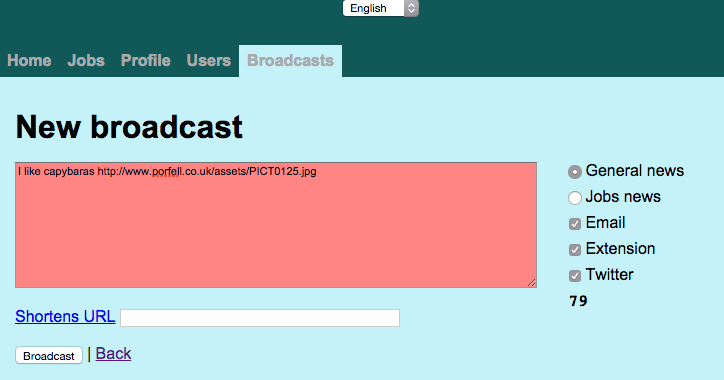
\includegraphics[width=0.75\textwidth]{createbc}
\caption{Creating a broadcast within the CSA application.}
\end{figure}

\newpage
Confirmation of the broadcast being created with the parameters that I gave on the previous screenshot is pictured in the screenshot that has been included below.\\
\\
You can see in the list of feeds that it includes the feed named 'Extension' which signifies that we want to alert users that are using the browser extension.

\begin{figure}[H]
\centering
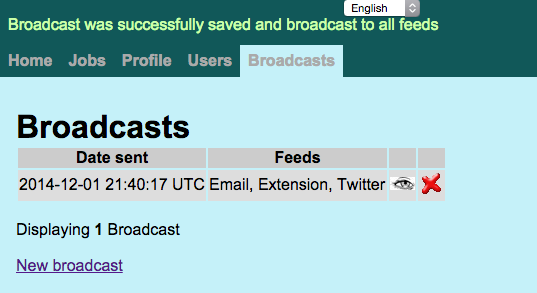
\includegraphics[width=0.75\textwidth]{confbc}
\caption{Here is the confirmation that a new broadcast has been created.}
\end{figure}

Here is shown a Chrome Notification for the broadcast that we just created. This notification will only be shown once when it has been created, then is stored and will not be shown again to the user which will prevent them from being annoyed by repeated notifications telling them the same information over and over.

\begin{figure}[H]
\centering

\includegraphics[width=0.5\textwidth]{chromenotification}
\caption{Here is a Chrome notification showing the latest broadcast.}
\end{figure}

Due to the nature of how the browser Opera is designed it users the same core frameworks as Chrome thus allowing it to use the same browser extensions without any modifications. The screenshot below shows the same broadcast that we created earlier also being displayed within Opera's notification system.

\begin{figure}[H]
\centering

\includegraphics[width=0.5\textwidth]{operanotification}
\caption{Same again but for Opera this time just to show multi platform support.}
\end{figure}

\newpage
Just to confirm that this is a real broadcast and has not broken any of the other functionality within the CS-Alumni application, this is a screenshot of the broadcast on the Twitter website.

\begin{figure}[H]
\centering
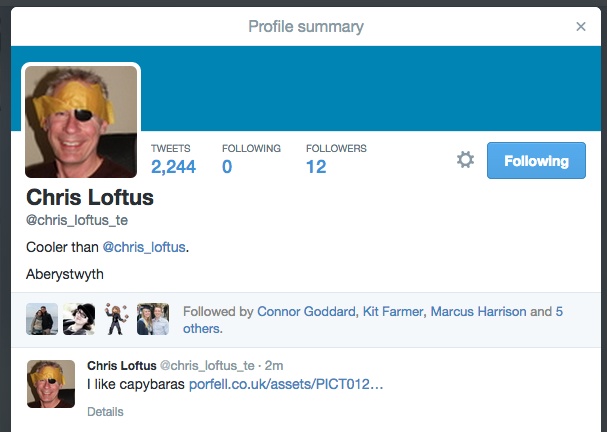
\includegraphics[width=0.8\textwidth]{twitterbc}
\caption{Proof that the broadcasts still get sent to Twitter.}
\end{figure}


\subsection{CS-Alumni Rails Application}

\subsubsection{New Additions}

\paragraph{New Database View}

\paragraph{New RESTful interface}

\subsubsection{Modifications}

\paragraph{Changes to Seeds}

\paragraph{Changes to Broadcasts}

\paragraph{Changes to Security}

\paragraph{Changes to REST implementation}

\paragraph{Changes to Users}

\paragraph{Changes to Tests}

\subsection{Communication Between Applications}

\subsubsection{RESTful Web Interfaces}

\subsubsection{Data Flow Diagrams}


%-- Application Testing.
\newpage
\section{Application Testing}

\subsection{Rails Unit Tests}

For testing the rails application I had to fix the functionality of the included tests to make them work with the rails application. Once theses changes had taken place it was possible to complete the tests successfully.\\
\\
One issue I have run into though is on first run of the \"rake test\" one of the tests will fail but on the second execution the tests will work perfectly. My theory behind this is that it is not guaranteed that the tests will run in order and that one of the other tests authenticates with the CS-Alimni application beforehand allowing the transaction to work as intended second time round.

\begin{figure}[H]
\centering
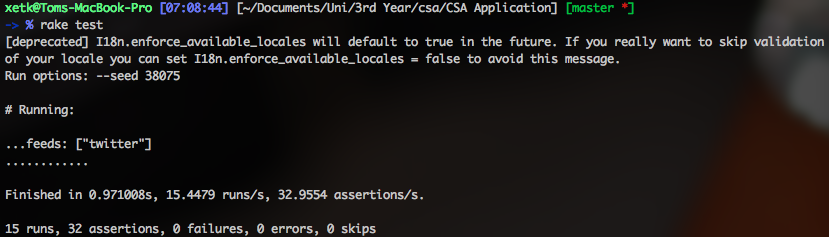
\includegraphics[width=\textwidth]{railstests}
\caption{This shows that the Ruby on Rails tests work successfully.}
\end{figure}

\subsection{QUnit Tests}

While developing my browser extension for this assignment I decided it was best to take a test driven style methodically to the design and construction of the extension, creating tests and then making the code that works with the test.\\
\\
I used an external JavaScript unit testing framework to allow the code to be tested efficiently. The framework I used was called QUnit and was developed by the same developers that created the other JavaScript library that I used called jQuery.\\
\\
For each of the libraries that I wrote to give the core functionality to the application I created their own page of tests. The results of the unit tests at the end of the project are pictured below.\\
\\
This is the class that handles all of the background interactions with the REST services. This creates notifications for new broadcasts being created.\\
\\
\begin{figure}[H]
\centering
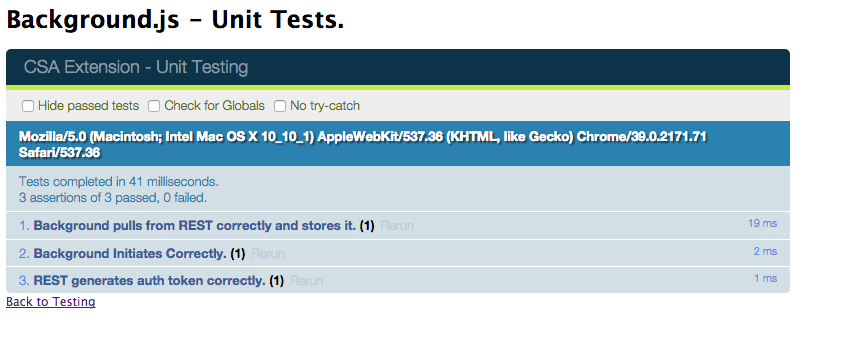
\includegraphics[width=\textwidth]{backgroundqunit}
\caption{This is the unit tests for the background.js module for the browser extension.}
\end{figure}

This library is used to get the version of the browser that is in use.\\

\begin{figure}[H]
\centering
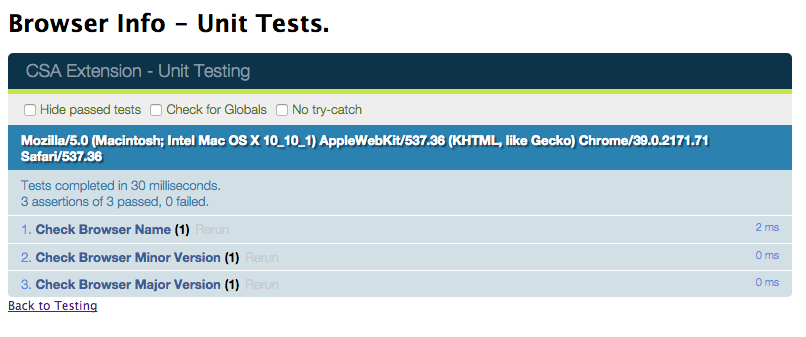
\includegraphics[width=\textwidth]{biqunit}
\caption{This image shows the browserinfo.js module completing its tests successfully.}
\end{figure}

Library for handling interaction with local storage.\\
\begin{figure}[H]
\centering
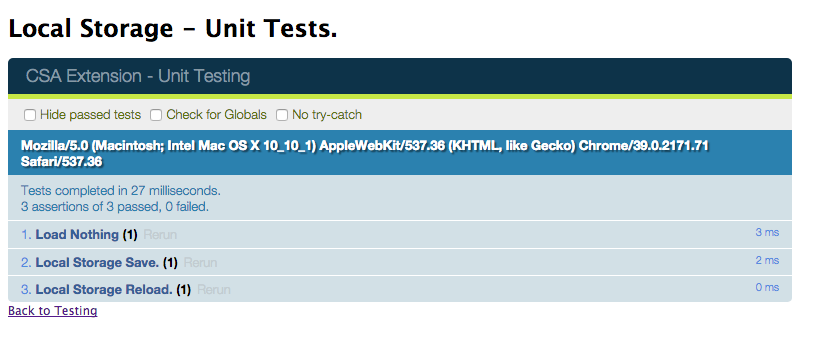
\includegraphics[width=\textwidth]{lsqunit}
\caption{This shows the LocalStorage.js module passing all its unit tests.}
\end{figure}

This is a wrapper around some of the AJAX methods within the jQuery library to make interaction with the server a little bit simpler.\\

\begin{figure}[H]
\centering
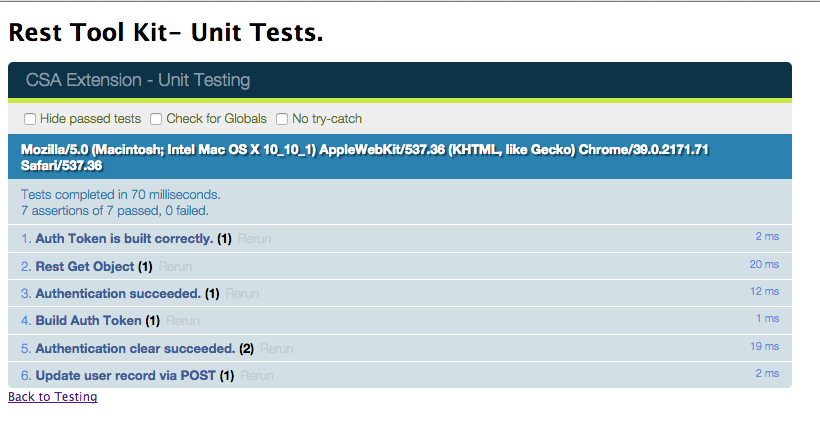
\includegraphics[width=\textwidth]{restqunit}
\caption{Above we see the RestToolKit.js module successfully completing all its unit tests.}
\end{figure}

This is a small utility library I have written to share commonly used functions between the various screens within the application.\\

\begin{figure}[H]
\centering
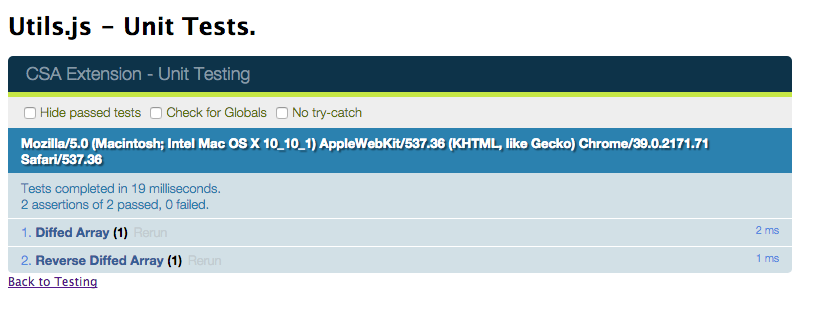
\includegraphics[width=\textwidth]{utilsqunit}
\caption{Included above we see the Utils.js module efficiently complete all of its unit tests.}
\end{figure}

%-- Technologies.
\section*{Technologies}

\subsection{CS-Alumni Chrome Browser Extension}

\subsubsection{HTML}

HTML is a markup language that dictates the layout of the screens that are shown within the browser extension it is the skeleton in which the content is placed and displayed to the end user, it has no style to start with it just is the structure of the screen.

\subsubsection{CSS}

CSS works tangent with HTML and gives the skeleton of a document some style, it is responsible for colour schemes along with the positioning of various elements on the page and how they are displayed.

\subsubsection{JavaScript}

Is the programing language that the browser extension has been written in, Google's definition for JavaScript is 'an object-oriented computer programming language commonly used to create interactive effects within web browsers.'.\\
\\
JavaScript is an integral part of creating an interactive experience for web based content. It interacts with the various libraries we require to make the application work as intended. It works together with the other web based web technologies within the browser extension to give us total control of the content that is presented on the screen.

\subsubsection{Chrome Extensions API}

This is the framework that we must adhere to to make the 3 main web based technologies (HTML, CSS and JavaScript) work as a browser extension, the Chrome Extensions API bundles all of the technologies we need to create a viable and fully working browser extension, it takes in the web technologies plus a few extra configuration files to generate a browser extension that will do what the developer intended.

\subsubsection{Bootstrap}

Bootstrap I see as an essential tool to creating a modern looking website, it unifies the appearance of the application along with giving the ability to make the pages adaptive and work on any screen size. This means that if we were to run the browser extension as a web page it would work on any screen size or any resolution.\\
\\
I choose to not use the standard Bootstrap theme opting to use a modified one that was supplied by \url{http://bootswatch.com/} (Theme name is Yeti) I choose to modify this further and make it try and more closely fit the Aberystwyth colour scheme.

\subsubsection{jQuery}

Along with Bootstrap I also see jQuery as an essential library to be able to create modern and feature full web applications (If I remember correctly all of the other JavaScript libraries I am using rely on jQuery).\\
\\
Within the application I use jQuery to handle many bits of the functionality within the screens, the key points being aJax requests this enables very simple REST type responses to the server without much hassle, I also use it to edit DOM elements in real time and make them display the information I want them to display in real time.\\
\\
The jQuery library is so vast that I use a lot of the trivial functions for doing all sorts of other work as the method calls and work that is required is greatly reduced.

\subsubsection{Moment.js}

This library simplifies interaction with date objects, its is well known that is quite difficult working with date objects within JavaScript, this library takes all the pain out of modifying the dates and putting them into a format that developer actually wants.\\
\\
I use it for the broadcast times to make them display in the correct way, the objects have been converted into a JSON string and when they are converted back they stay as a string I use moment to convert theses strings into a viable date object that then can be displayed on the screen.

\subsubsection{Alertify.js}

Alertify is a JavaScript library that makes modern user alerts, this gives well designed and easy to use dialogs to present information to the user.\\
\\ 
I have used it within the application to notify when a user has not been logged in and redirect them to the login page, along with showing a message confirming that there settings have been saved successfully.

\subsubsection{Qunit}

Due to doing a test driving development strategy to developing this browser extension I needed a unit test framework for JavaScript, it is developed by the same developers as jQuery and seems to have strong industry recognition.\\
\\
I have used this for all my unit testing for the JavaScript libraries that I have written for this project, It has a simple and efficient way of testing the functions along with having a simple and powerful syntax that allows tests to be written without much code.

\subsection{CS-Alumni Rails Application}

\subsubsection{Ruby}

Ruby is a object orientated program language that is dynamically typed which means there is no strict types for objects

\subsubsection{Ruby on rails}

Ruby on Rails (RoR) is a web framework that allows the use of the Ruby programing language to create web based applications, it has a strong modularity and is easily extended through the use of Ruby Gems which are small library that can be imported to allow extra functionality within the project.

The CS-Alumni application that we were given as a starting 

\subsubsection{Rack Middleware}

\subsection{Communication Between Applications}

\subsubsection{RESTful Interfaces}

\subsubsection{CORS}

\subsubsection{Basic Authentication}

%-- Evaluation.
\newpage
\section{Evaluation}

\iffalse
 _________    ________      ________      ________     
|\___   ___\ |\   __  \    |\   ___ \    |\   __  \    
\|___ \  \_| \ \  \|\  \   \ \  \_|\ \   \ \  \|\  \   
     \ \  \   \ \  \\\  \   \ \  \ \\ \   \ \  \\\  \  
      \ \  \   \ \  \\\  \   \ \  \_\\ \   \ \  \\\  \ 
       \ \__\   \ \_______\   \ \_______\   \ \_______\
        \|__|    \|_______|    \|_______|    \|_______|       


                                                            .-'
                                                         .-'
                                                      .-'
                                                   .-'
                                                .-'
                  /)                         .-'
                 ||                       .-'
                 ||                    .-'
                 ||                 .-'
                 ||              .-'     .------.
                 ||           .-'  __   | *meow* |
                 ||        .-'   .'-/__ |  _.---'
                 |`-------------'    \/ /.'
                 |*                 '| /'
                 |     |          `--'
               .-| |  /_______    |
            .-'  | | <        `.|||               _.'|
         .-'____  \\`.`.       ||||           _.-'_.-|
      .-'  ||   `--`- `.).____ ||||       _.-'_.-'   |
   .-'     ||                 ``-``--._.-'_.-'       |
.-'        ||                         |`-'           |
           ||                         | |            |
           ||                         | |            |
           ||                         | |            |
           ||                         | |            |
           ||                         | |            |
           ||                        |`--;}};.       |
           ||                       .'  o\ }}}}      |
           ||                     .'\      }}}}      |
           ||                     |      )}}}}}      |
           ||                      \    '}}}}}       |
           ||                       L    }}}}}}      |
           ||                       |  _.}}}}}}      |
           ||                    .-'|.'.-`-}}}}}     |
           ||                  .'  |/|/      `.}}    |
           ||                .' /              \}    |
           ||               /  |           \    \    |
           ||              /   |           |\    \   |
           ||            .'   .'\          | \    \  |
           ||          .'   .'  |   `      |  \    \ |
`.         ||        .'   .'    |          |   |    )|
  `.       ||     .-'\  .'      |          (  /   .' |
    `.     ||   _/__.'`'        J          J /   /   |
      `.   || (')               |           /   /    | 
        `. ||                   F          <   /     |
          `||                   L        ,/ `./      |
           ||                   `-.__.---/'_/_/      |
           ||                   |       //-'|        |
           ||                   |      //   |        |
           ||                   |      '    |        |
           ||                   |           |        |
           ||                   `-.______.-'         |
           ||                    |    F    |         |
           ||                    (   J|    F         |
           ||                    |   ||   J          |
           ||                    |   |J(   L         |
           ||                    J   F|F   |         |
           ||                    |  J ||   |         |
           ||                    |  |_||   F         |
           ||                   _F  J `|  J          |
           ||               _.-'/_.' ) |  |`.        |
           ||           _.-' .-'  /\/  |  |. `.      |
           ||       _.-'     `---'     F  ) `. `.    |
           ||   _.-'                  /-'/|   `. `.  |
           ||.-'                    .__.'       `. `.|
                                                  `. |
                                                    `|
                                                      `.
  VK                                                    `.
                                                          `.


\fi   

\newpage
\section{Something Extra}
%-- Talk about pebble app here.
\begin{figure}[H]
\centering
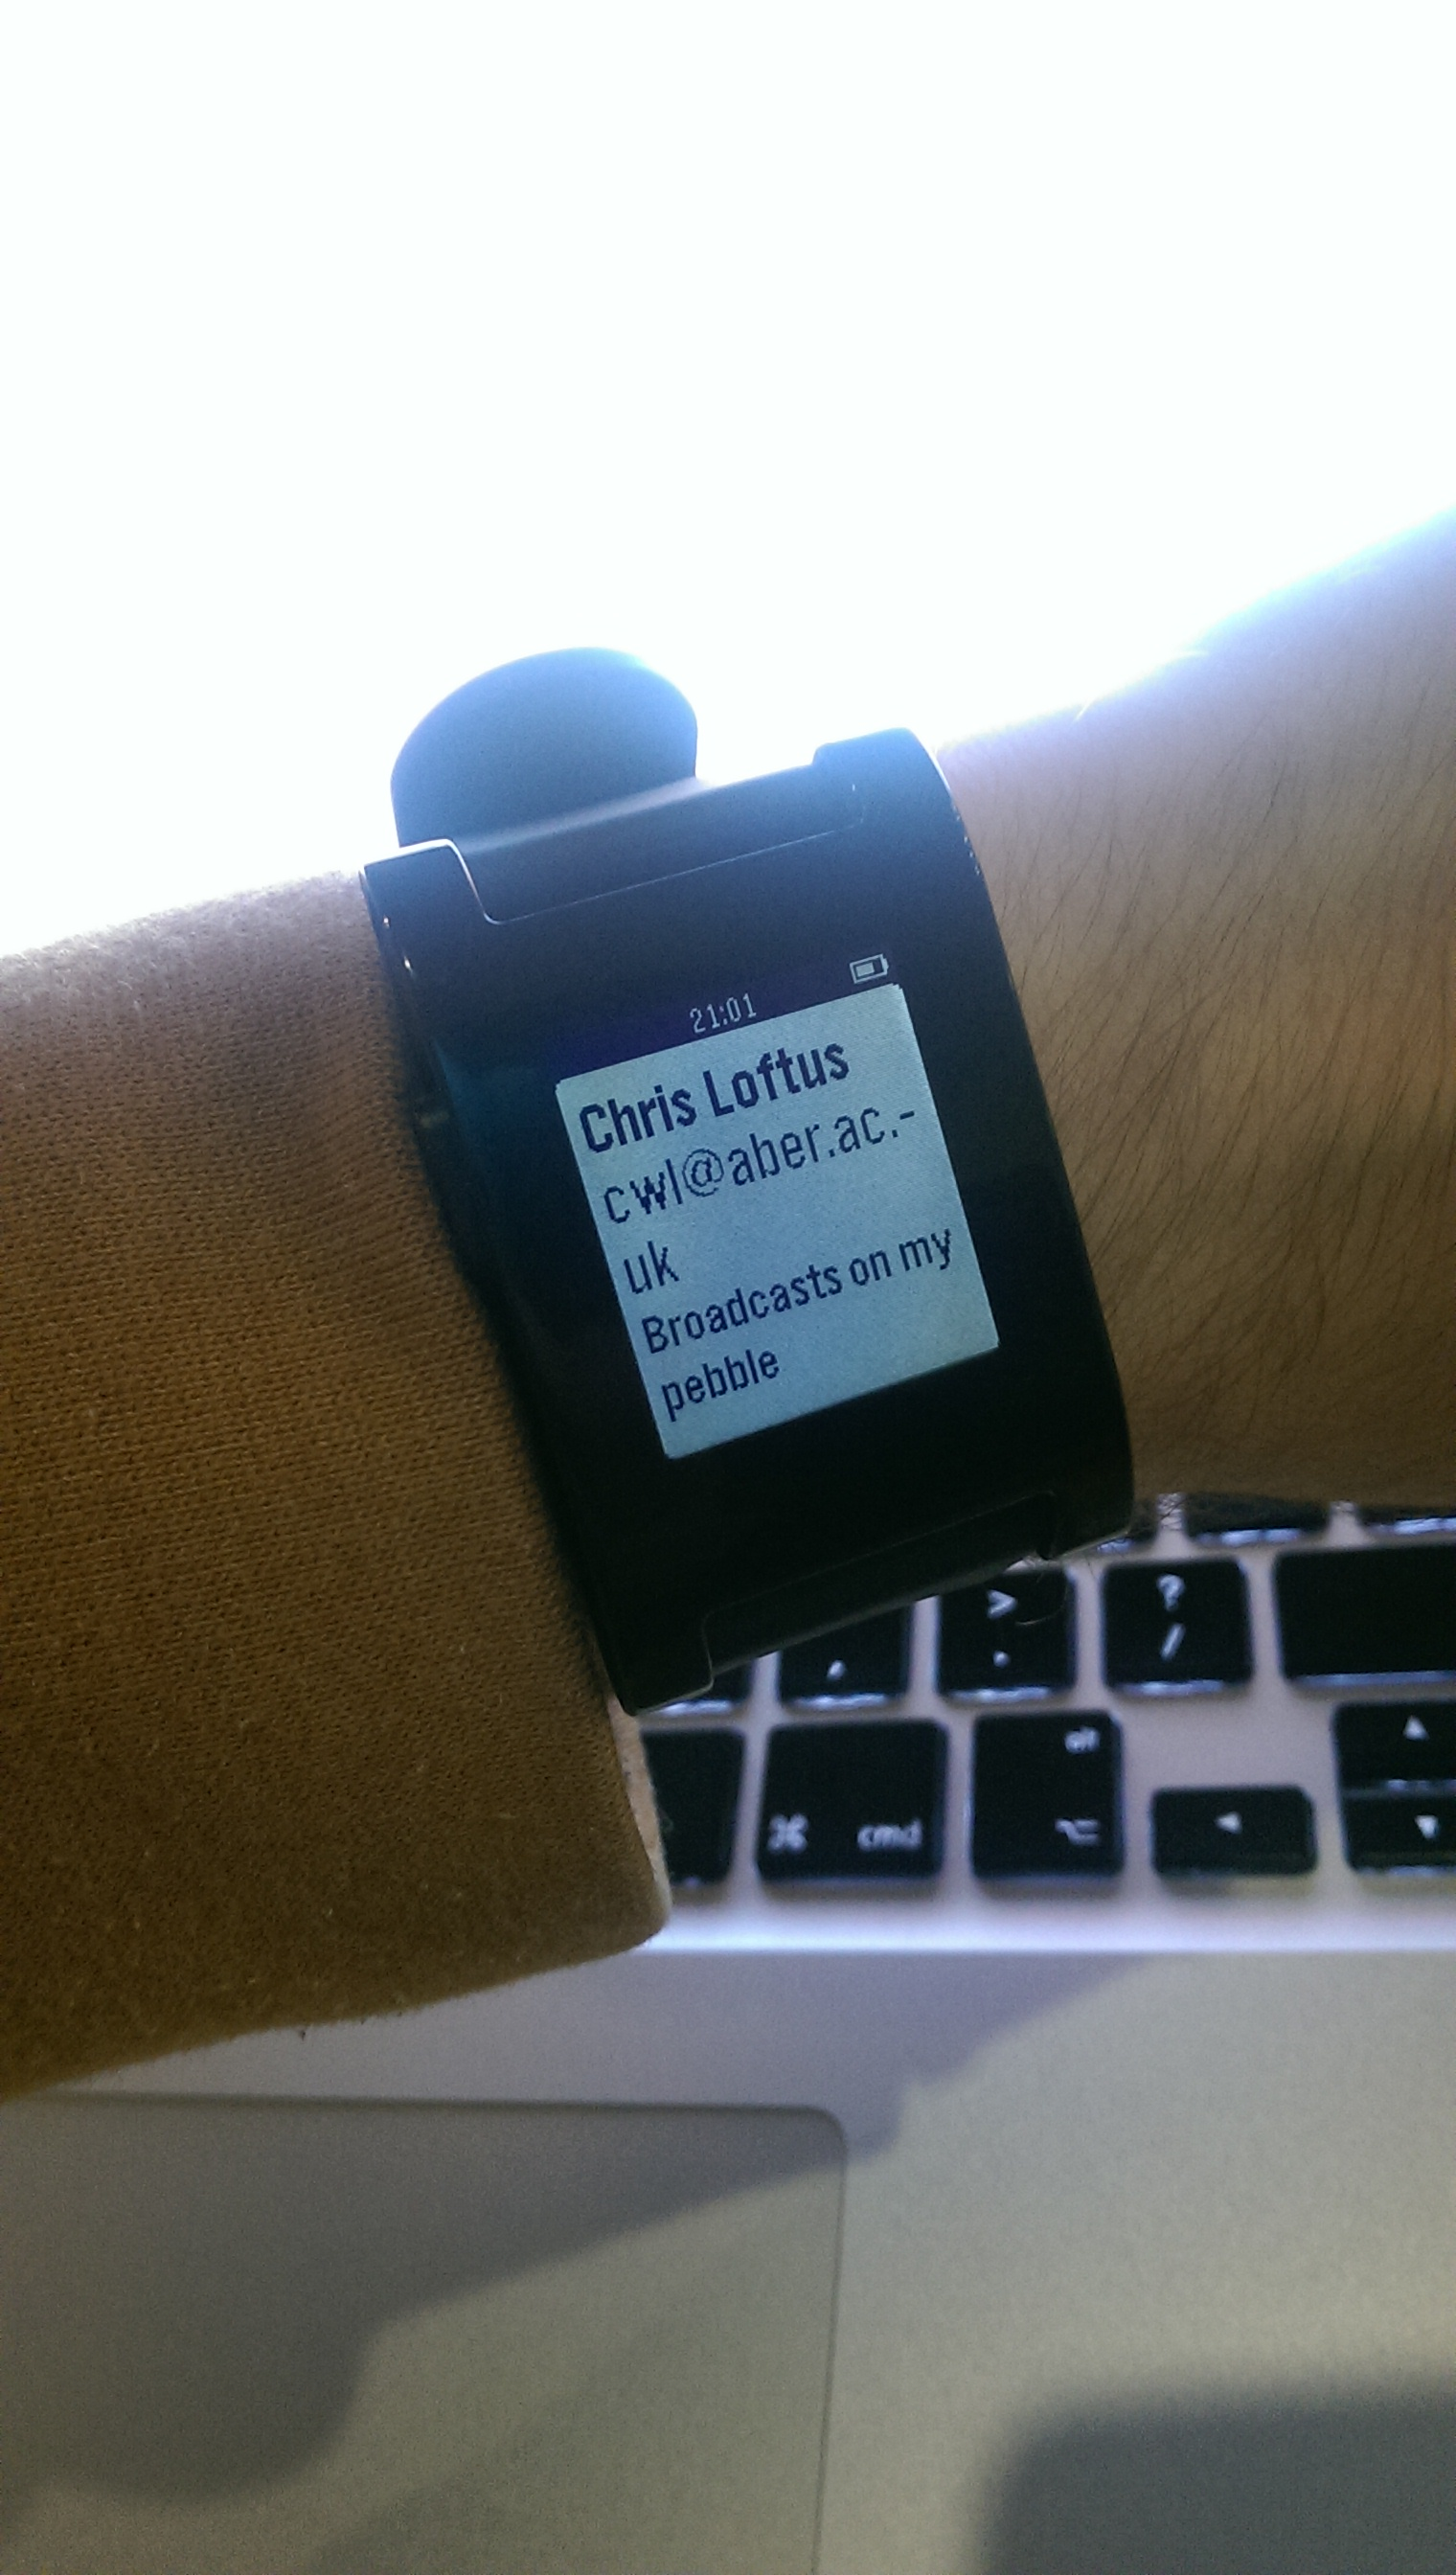
\includegraphics[width=0.5\textwidth]{pebble}
\caption{Above is a image of the Pebble smartwatch running the CSA application.}
\end{figure}

\begin{figure}[H]
\centering
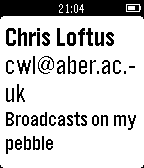
\includegraphics[width=0.25\textwidth]{pebblesh}
\caption{This is a screenshot taken from the Pebble smartwatch.}
\end{figure}

\newpage
%-- Attributions.
\section*{Attributions}

\newpage
\printbibliography

\end{document}